%
%
%		Finding: Template
%		Author: the DR
%
%
\renewcommand{\FindingAuthor}{Michal Olencin}
% DO NOT USE \par, \newline or any other line breaking command in FindingName => report will not build
\renewcommand{\FindingName}{Outdated Components}
\renewcommand{\Location}{dummyapplication.apk, dummyapplication.ipa}
\renewcommand{\Component}{Multiple}
\renewcommand{\FoundWith}{Manual testing}
\renewcommand{\TestMethod}{Manual}
\renewcommand{\CVSS}{2.5}
\renewcommand{\CVSSvector}{CVSS:3.1/AV:L/AC:H/PR:L/UI:N/S:U/C:L/I:N/A:N}
\renewcommand{\CWE}{1104}
% Poor-man's combo boxes:
% High, Medium, Low, Info, TBR (To Be Rated)
\renewcommand{\Criticality}{Low}
% Easy, Average, Hard, TBR (To Be Rated)
\renewcommand{\Exploitability}{Hard}
% Access control, Application Design, Information Disclosure, Outdated Software, Security Configuration
\renewcommand{\Category}{Outdated Software}
% Easy, Average, Difficult, TBR (To Be Rated)
\renewcommand{\Detectability}{Easy}


\ReportFindingHeader{\FindingName}


%-------------------------------------------
%	Details                                |
%-------------------------------------------

\subsection*{Details}

The application uses outdated third party components.
Also the application uses API level 21 (Android 5.0) as minimum API level required for the application to run.


%-<Details>
%-------------------------------------------
%	Impact                                 |
%-------------------------------------------

\subsection*{Impact}

Outdated third party components can compromise the security of an application, leading to data theft, business disruption, legal issues, and harm to reputation.
Upgrading these packages and monitoring the system's security is necessary to avoid these consequences.
The best practice is to use the latest versions of components.

By setting the minimum API level to 21, the application can be installed on an older version of Android that has multiple unfixed vulnerabilities.
This increases the risk of known vulnerabilities in older Android versions being exploited by attackers, potentially compromising the security of the application and user data.

%-<Impact>
%-------------------------------------------
%	Repeatability                          |
%-------------------------------------------
\subsection*{Repeatability}

Observe the set value \texttt{minSdkVersion} in the file \texttt{build.gradle} to check Android minimum API level (see \cref{figure:gradle}).

\begin{figure}[H]
\centering
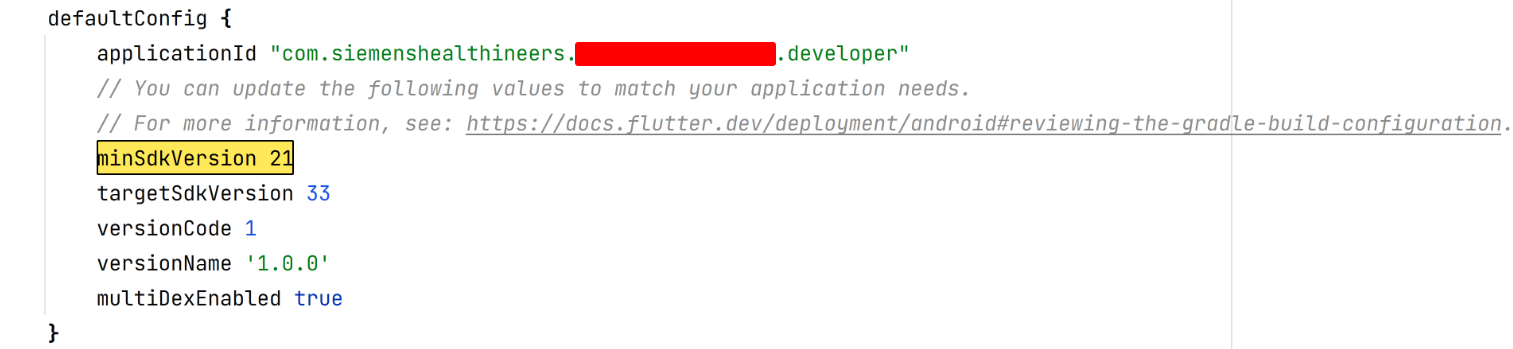
\includegraphics[width=0.9\textwidth,frame]{\CurrentFilePath/gradle.png}
\caption{Snippet of the \texttt{build.gradle} file}
\label{figure:gradle}
\end{figure}

Observe the output of the command \texttt{flutter pub outdated} to check outdated third party components (see \cref{figure:flutter}).

\begin{figure}[H]
\centering
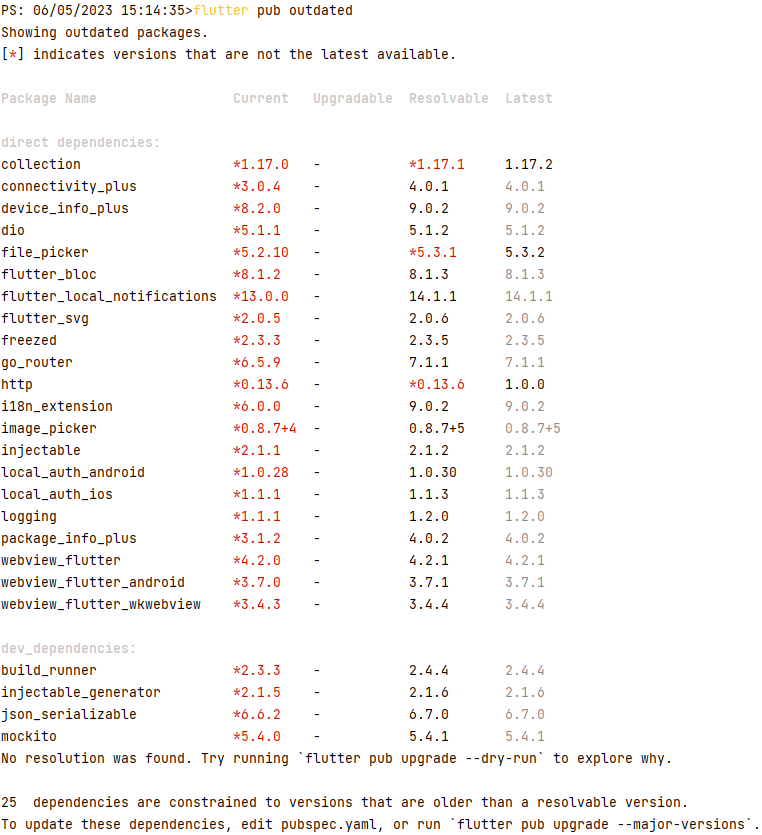
\includegraphics[width=0.9\textwidth,frame]{\CurrentFilePath/flutter.png}
\caption{Output of the command \texttt{flutter pub outdated}}
\label{figure:flutter}
\end{figure}
 
%-<Repeatability>
%-------------------------------------------
%	Countermeasures                        |
%-------------------------------------------
\pagebreak
\subsection*{Countermeasures}

The following countermeasures are recommended:

\begin{itemize}
    \item Review all used libraries for vulnerable versions and upgrade the outdated ones.
    \item Consider signing up to \href{https://svm.cert.siemens.com/portal/}{Security Vulnerability Monitoring}.
    \item Perform regular updates of used components.
    \item Increase Android minimum API level. Setting API level 29 (Android 10) is recommended.
\end{itemize}

%-<Countermeasures>
%-------------------------------------------
%	References - pulls bib entries         |
%-------------------------------------------

\subsection*{References}

This finding references the following information sources:

\begin{itemize}
    \item \href{https://svm.cert.siemens.com/portal/}{Security Vulnerability Monitoring}
	\item \href{https://www.first.org/cvss/calculator/3.1#CVSS:3.1/AV:L/AC:H/PR:L/UI:N/S:U/C:L/I:N/A:N}{CVSS 2.5}
	\item \bibentry{CWE-1104}
\end{itemize}

%-<References>

